% Document setup----------------------------------------------------------------
\documentclass[10pt, xcolor=dvipsnames,compress]{beamer}
\usetheme{Berlin}

% Presentation setup------------------------------------------------------------
\setbeamertemplate{footline}[frame number] % Include page number
\beamertemplatenavigationsymbolsempty      % Remove navigation bar
\usecolortheme{metropolis}

\setbeamercolor{background canvas}{bg=white}
\setbeamercolor{titlelike}{bg=white}
\setbeamercolor{titlelike}{bg=white}
\setbeamercolor{author}{bg=white}
\setbeamercolor{institute}{bg=white}
\setbeamercolor{date}{bg=white}

% Title page in sections -------------------------------------------------------
\AtBeginSection[]{
  \begin{frame}
    \vfill
    \centering
    \begin{beamercolorbox}[sep=8pt,center,shadow=false,rounded=true]{title}
        \usebeamerfont{title}\insertsectionhead\par
    \end{beamercolorbox}
    \vfill
  \end{frame}
}

% Import packages---------------------------------------------------------------
% Aesthetics packages ----------------------------------------------------------
\usepackage{amsfonts}

% Aesthetic commands -----------------------------------------------------------
\definecolor{marineblue2}{rgb}{0.05,0.1,0.5}

% Math packages ----------------------------------------------------------------
\usepackage{amsmath}
\usepackage{bbm}

% Referencing packages ---------------------------------------------------------
\usepackage{hyperref}

% Math commands ----------------------------------------------------------------
\newcommand{\N}{\mathbb{N}}
\newcommand{\Z}{\mathbb{Z}}
\newcommand{\R}{\mathbb{R}}


% Define title -----------------------------------------------------------------
\title{P218 Econometrics I}
\subtitle{TA Session 2}
\author{Gabriel Simões Gaspar}
\institute{London Business School}
\date{Fall 2022}

% Start document ---------------------------------------------------------------
\begin{document}

% Title frame ------------------------------------------------------------------
\maketitle

% Outline frame ----------------------------------------------------------------
\begin{frame}{Roadmap}
    \tableofcontents
\end{frame}

% Gauss-Markov recap section ---------------------------------------------------
% Begin section ----------------------------------------------------------------
\section{Gauss-Markov Theorem}

% Classical GM subsection ------------------------------------------------------
\subsection{The Gauss-Markov Theorem}

\begin{frame}{Gauss-Markov Theorem}

    In lecture you saw the famous Gauss-Markov Theorem. Consider the linear regression model described by
    \begin{align*}
        Y &= X \beta + \varepsilon
        \\
        \mathbb{E}[\varepsilon \mid X] &= 0
        \\
        \operatorname{Var}(\varepsilon \mid X) &= \mathbb{E}[\varepsilon \varepsilon' \mid X] = \sigma^2 \Sigma < \infty
    \end{align*}
    where $Y$ is an $n \times 1$ random vector, $X$ is an $n \times m$ full-rank matrix of regressors such that $m < n$ and $\varepsilon$ is an $n \times 1$ vector of regression errors.

    \vspace{2em}

    If we add the assumption that the variance-covariance matrix $\Sigma = I_n$, then you saw that the OLS estimator has \textbf{minimum variance} among the estimators that (\textbf{conditional} on regressors) are \textbf{linear} and \textbf{unbiased}. This is famously known as the best linear conditionally unbiased estimator, i.e. BLUE.

\end{frame}

\begin{frame}{Gauss-Markov Assumptions}

    We will summarise the conditions that make the OLS estimator BLUE as follows:
    \begin{align*}
        (GM0)& \qquad Y = X \beta + \varepsilon
        \\
        (GM1)& \qquad \text{rank}(X) = m 
        \\
        (GM2)& \qquad \mathbb{E}[Y \mid X] = X \beta \iff \mathbb{E}[\varepsilon \mid X] = 0
        \\
        (GM3)& \qquad \operatorname{Var}(Y \mid X) = \operatorname{Var}(\varepsilon \mid X) = \sigma^2 I 
    \end{align*}

    These are enough for us to prove the Gauss-Markov theorem. Let's quickly go over them.

\end{frame}

\begin{frame}{Unbiasedness}

    To show that the OLS is conditionally unbiased, simply note that
    \begin{align*}
        \hat{\beta}_{OLS} &\overset{GM1}{=} (X'X)^{-1} X'Y
        \\
        \hat{\beta}_{OLS} &\overset{GM0}{=} \beta + (X'X)^{-1} X' \varepsilon
    \end{align*}
    
    We can take the expectation on both sides of the equation above noting that $\mathbb{E} [\beta \mid X] = \beta$
    \begin{align*}
        \mathbb{E} [ \hat{\beta}_{OLS} \mid X] &= \beta + \mathbb{E} [ (X'X)^{-1} X'(\varepsilon) \mid X]
        \\
        \mathbb{E} [ \hat{\beta}_{OLS} \mid X] &= \beta + (X'X)^{-1} X' \mathbb{E} [ \varepsilon \mid X]
    \end{align*}
    
    which finally shows us that:
    \begin{align*}
        \mathbb{E} [ \hat{\beta}_{OLS} \mid X] &\overset{GM2}{=} \beta
    \end{align*}

\end{frame}

\begin{frame}{Minimum Variance}

    Imagine now a general-form \textbf{unbiased linear} estimator $\tilde{\beta}$ for $\beta$ that follows $(GM0)$ - $(GM3)$ defined as follows:
    \begin{align*}
        \tilde{\beta} = AY \overset{GM0}{=} A(X \beta + \varepsilon) \implies \mathbb{E}[\tilde{\beta} \mid X] \overset{GM2}{=} AX \beta = \beta \implies AX = I_n
    \end{align*}
    
    The conditional variance of this estimator is simply:
    \begin{align*}
        \operatorname{Var} (\tilde{\beta} \mid X) &= A \operatorname{Var} ( Y \mid X) A' \overset{GM3}{=} \sigma^2 A A'
    \end{align*}
    
    We can decompose the general matrix $A$ by adding and subtracting another matrix:
    \begin{align*}
        A = A - \underbrace{ (X'X)^{-1} X' + (X'X)^{-1} X'}_{=0} = W + (X'X)^{-1} X'
    \end{align*}

    where we have defined $W \equiv A - (X'X)^{-1} X'$.

\end{frame}

\begin{frame}{Minimum Variance}

    Note that:
    \begin{align*}
        W \equiv A - (X'X)^{-1} X' \implies W X = \underbrace{AX}_{= I_n} - \underbrace{(X'X)^{-1} X' X}_{I_n} = 0
    \end{align*}

    Plug in the decomposed $A$ we derived in the previous slide in the conditional variance:
    \begin{align*}
        \operatorname{Var} (\tilde{\beta} \mid X) &= \sigma^2 A A'
        \\
        &= \sigma^2 (W + (X'X)^{-1} X') (W' + X (X'X)^{-1} )
        \\
        &= \sigma^2 [W W' + \underbrace{W X}_{=0} (X'X)^{-1} + (X'X)^{-1} \underbrace{X' W'}_{(WX)'=0} + (X'X)^{-1} ]
        \\
        &= \sigma^2 WW' + \sigma^2 (X'X)^{-1}
        \\
        &> \sigma^2 (X'X)^{-1}
        \\
        &= \operatorname{Var}(\hat{\beta}_{OLS} \mid X)
    \end{align*}
    
\end{frame}

\begin{frame}{General Var-Cov Matrix}

    Let's now make a slight change and consider a model such that:
    \begin{align*}
        (GM3') \qquad \operatorname{Var}(\varepsilon \mid X) = \mathbb{E}[ \varepsilon \varepsilon' \mid X] = \Omega < \infty
    \end{align*}

    so we are not (necessarily) considering the homoskedastic case anymore. What is the variance of the OLS estimator in this case?
    \begin{align*}
        \operatorname{Var}(\hat{\beta}_{OLS} \mid X ) &\overset{GM1}{=} \operatorname{Var}( (X'X)^{-1} X' Y \mid X)
        \\
        \operatorname{Var}(\hat{\beta}_{OLS} \mid X ) &\overset{GM0}{=} (X'X)^{-1} X' \operatorname{Var}( \varepsilon \mid X) X (X'X)^{-1}
        \\
        \operatorname{Var}(\hat{\beta}_{OLS} \mid X ) &\overset{GM3'}{=} (X'X)^{-1} X' \Omega X (X'X)^{-1}
    \end{align*}
    
    Is OLS best in this case? We will see this later in the course.
    
\end{frame}


% Question 1 section -----------------------------------------------------------
% Begin section ----------------------------------------------------------------
\section{Question 1}

% Part (a) ---------------------------------------------------------------------
\begin{frame}{Part (a)}

    We have that:
    \begin{align*}
        Y = -X^2 + (2 + \varepsilon) X
    \end{align*}
    
    The effect of a marginal change of $X$ in $Y$ is simply:
    \begin{align*}
        \frac{\partial Y}{\partial X} = -2 X + (2 + \varepsilon)
    \end{align*}

    These effects are heterogeneous. Farms with good soil will have $\varepsilon = 1$, and so the marginal effect is $-2 X + 3$. Farms with bad soil have $\varepsilon = -1$ and so the marginal effect is $- 2X + 1$.
\end{frame}

% Part (b) ---------------------------------------------------------------------
\begin{frame}{Part (b)}

    To find the $ACE$ of $X$ on $Y$ as a function of $X$ we have to integrate out $\varepsilon$. This can be done in two steps. First, find the marginal density of $X$:
    \begin{align*}
        f_X(x) &= \int_{-1}^1 f_{X \varepsilon}(x, z) d z
        \\
        &= \int_{-1}^1 \frac{1 + x - z}{8} dz
        \\
        &= \varepsilon \Biggr( \frac{1 + x}{8} \Biggr) - \frac{z^2}{16} \Biggr |_{z=-1}^{z=1}
        \\
        &= \frac{1 + x}{4}
    \end{align*}

\end{frame}

\begin{frame}{Part (b)}

    Now that we have the marginal density of $X$, we can calculate the conditional density:
    \begin{align*}
        f_{\varepsilon \mid X}(z \mid x) &= \frac{f_{X \varepsilon} (x, z) }{f_X (x)}
        \\
        &= \frac{1 + x - z}{2 + 2x}
    \end{align*}

    Finally, the $ACE$ is then:
    \begin{align*}
        ACE(X) &= \int_{-1}^1 (- 2 x + 2 + z) \Biggr( \frac{1 + x - z}{2 + 2x} \Biggr) dz
        \\
        &= \frac{5 - 6X^2}{3X + 3}
    \end{align*}

\end{frame}

\begin{frame}{Part (b)}

    \begin{figure}[ht]
        \centering
        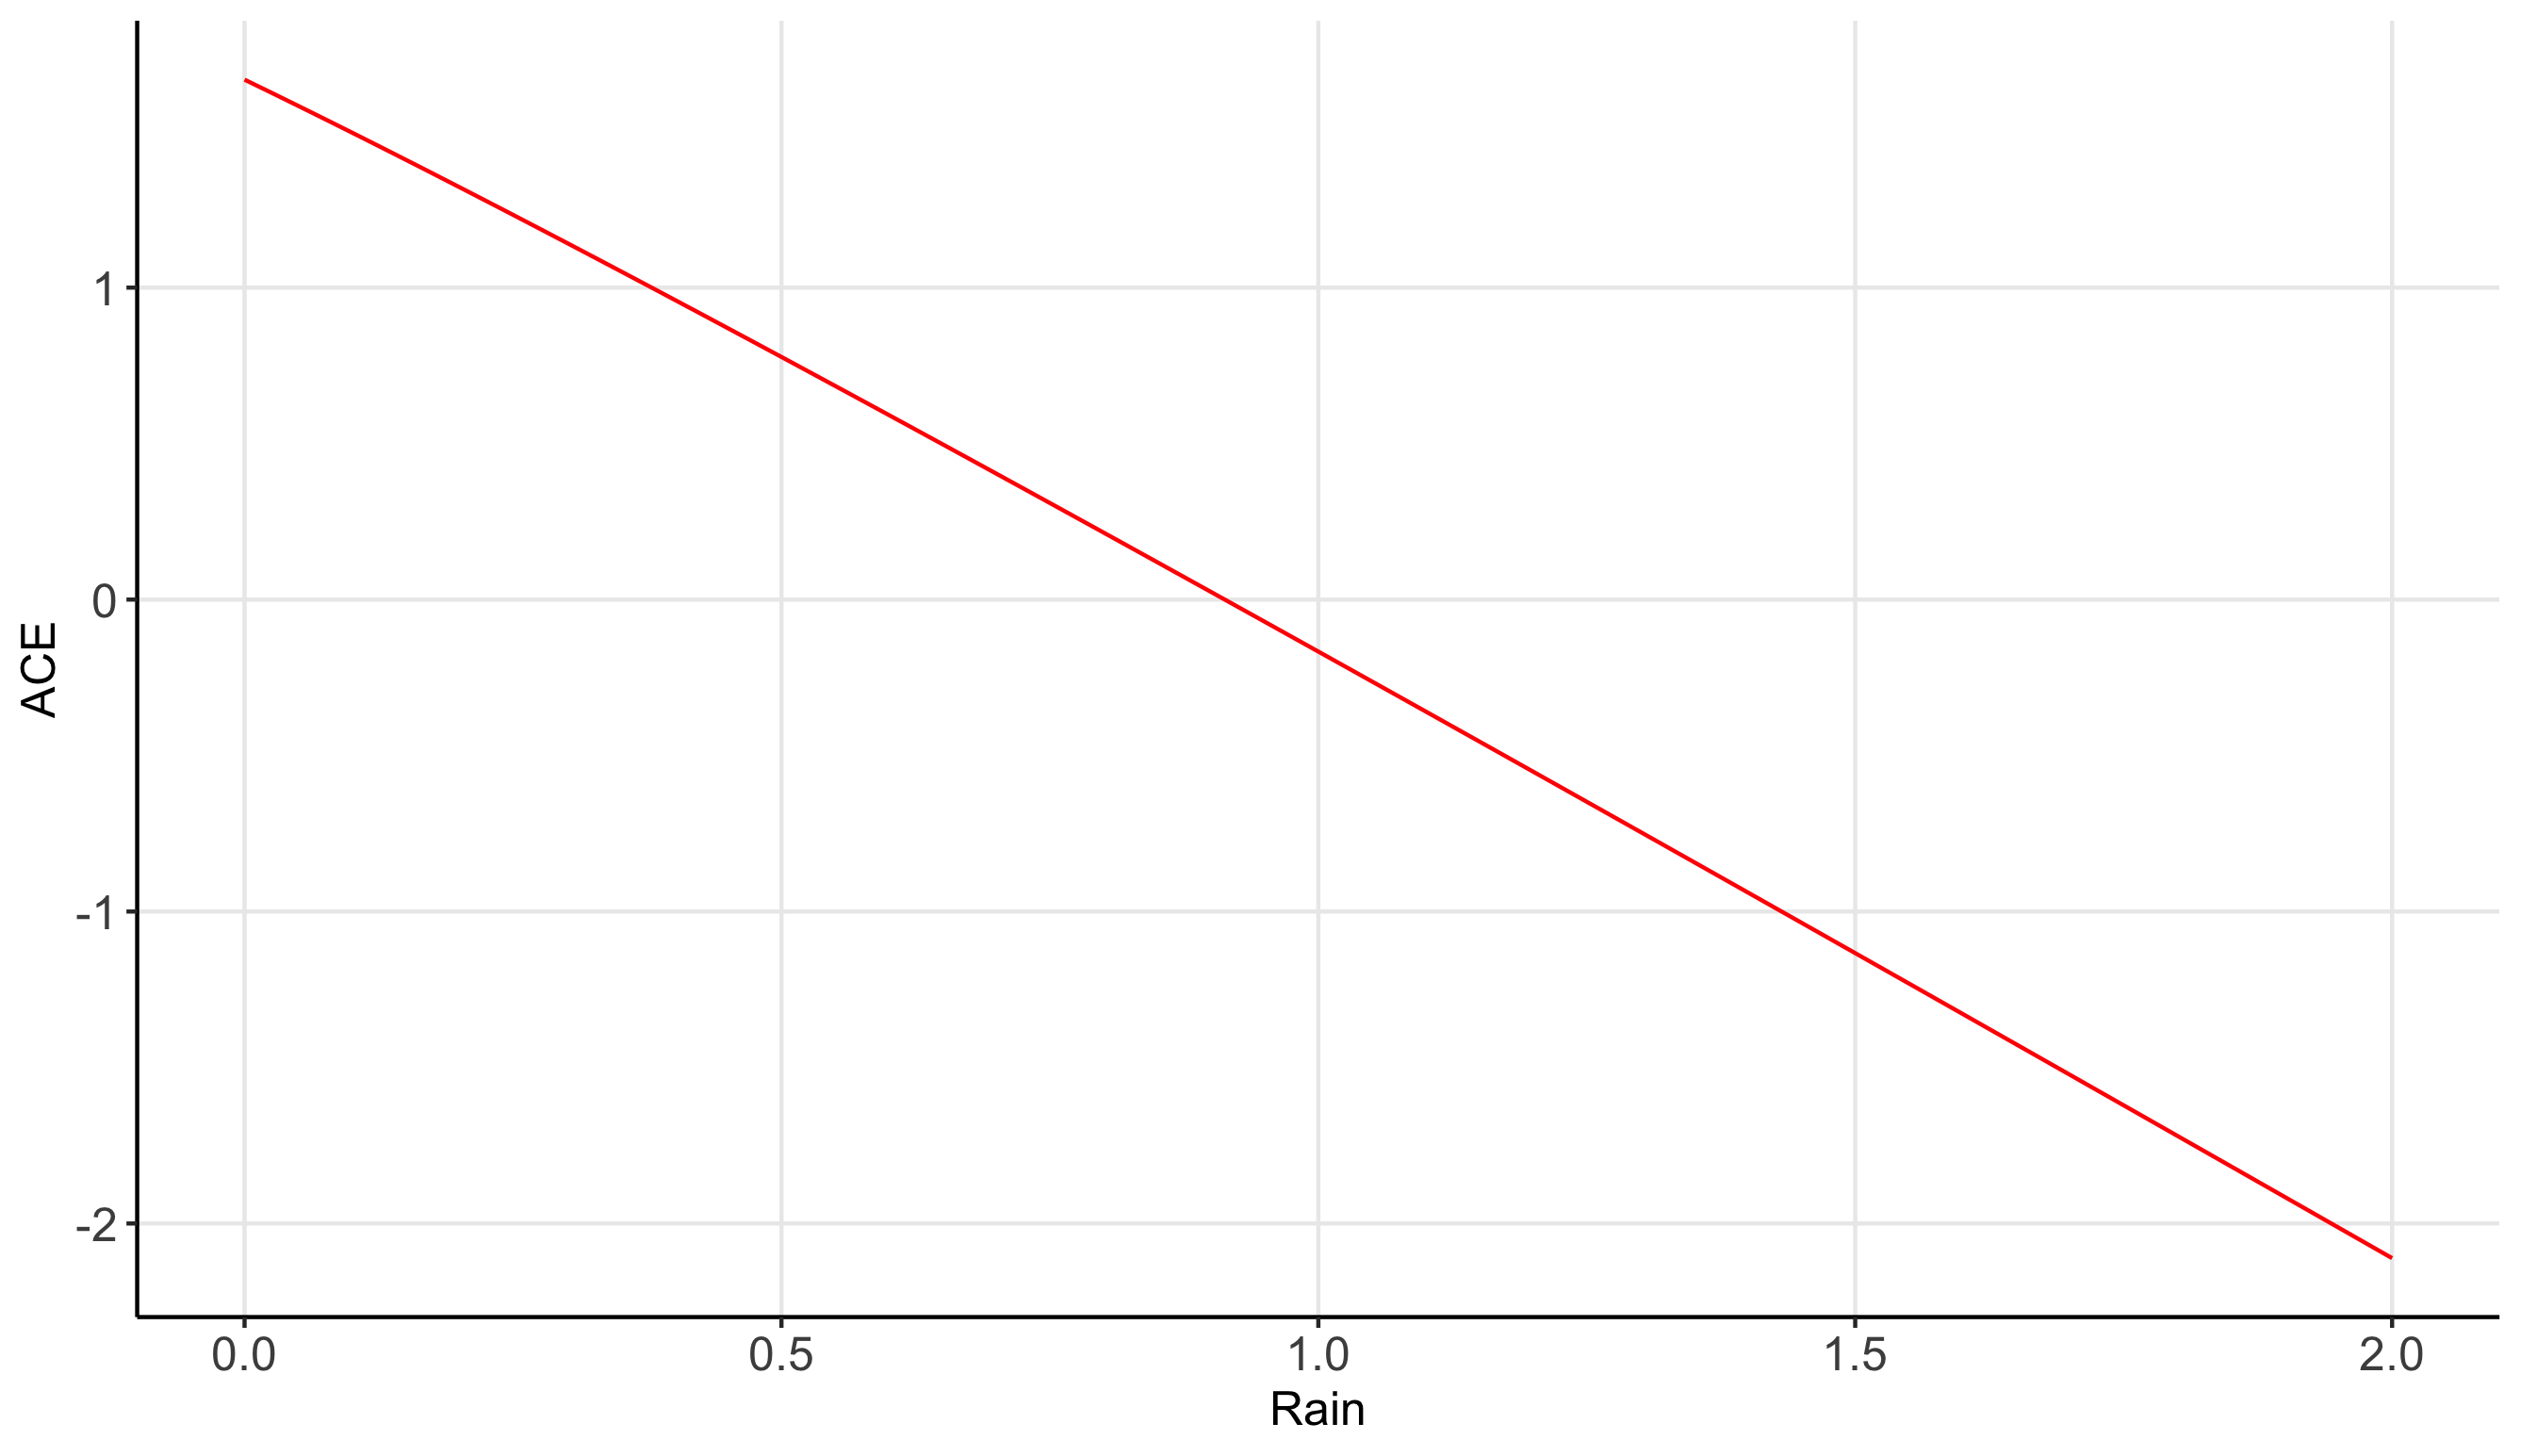
\includegraphics[width=1.0\linewidth]{./resources/question-1-b.png}
    \end{figure}

\end{frame}

% Part (c) ---------------------------------------------------------------------
\begin{frame}{Part (c)}

    To find the unconditional expectation just proceed as usual for a continuous variable:
    \begin{align*}
        \mathbb{E}[Y] &= \mathbb{E}[-X^2 + (2 + \varepsilon) X]
        \\
        &= \int_0^2 \int_{-1}^1 (-x^2 + (2 + z) x) f_{X \varepsilon}(x, z) dz dx
        \\
        &= \int_0^2 \int_{-1}^1 (-x^2 + (2 + z) x) \frac{1 + x - z}{8} dz dx
        \\
        &= \frac{1}{2}
    \end{align*}

\end{frame}

\begin{frame}{Part (c)}

    And the conditional mean:
    \begin{align*}
        \mathbb{E}[Y \mid X] &= \mathbb{E}[-X^2 + (2 + \varepsilon) X \mid X]
        \\
        &= -X^2 + X \mathbb{E}[ (2 + \varepsilon) \mid X]
        \\
        &= -X^2 + X \int_{-1}^1 (2 + z) f_{\varepsilon \mid X}(z \mid x) dz
        \\
        &= -X^2 + X \int_{-1}^1 (2 + z) \Biggr( \frac{1 + X - z}{2 + 2X} \Biggr) dz
        \\
        &= -X^2 + X \frac{6X  + 5}{3X + 3}
    \end{align*}

\end{frame}

\begin{frame}{Part (c)}

    In case you were skeptical about the Law of Iterated Expectations:
    \begin{align*}
        \mathbb{E}[Y] &= \mathbb{E}[ \mathbb{E}[Y \mid X] ]
        \\
        &= \int_0^2 f_X(x) \mathbb{E}[Y \mid X] dx
        \\
        &= \int_0^2 \Biggr( \frac{1+x}{4} \Biggr) \Biggr( -X^2 + X \frac{6X  + 5}{3X + 3} \Biggr) dx
        \\
        &= \frac{1}{2}
    \end{align*}

\end{frame}

% Part (d) ---------------------------------------------------------------------
\begin{frame}{Part (d)}

    Note that
    \begin{align*}
        \frac{\partial}{\partial X} \mathbb{E}[Y \mid X] = -2X + \frac{6X^2 + 12X + 5}{3(X + 1)^2} > \frac{5 - 6x^2}{3(x + 1)} = ACE(X)
    \end{align*}

    We can see that:
    \begin{align*}
        \frac{\partial}{\partial X} \mathbb{E}[Y \mid X] - ACE(X) &= -2X + \frac{6X^2 + 12X + 5}{3(X + 1)^2} - \frac{5 - 6x^2}{3(x + 1)}
        \\
        &= \frac{X}{3(x + 1)^2} > 0
    \end{align*}

    This means that the slope of the regression overstates the causal effect of rain $X$. Why does this happen? What is the CEF capturing?

\end{frame}

% Part (e) ---------------------------------------------------------------------
\begin{frame}{Part (e)}

    Let's do this by parts. We can calculate the variance of $X$ as:
    \begin{align*}
        \operatorname{Var}(X) &= \mathbb{E}[X^2] - \mathbb{E}[X]^2
        \\
        &= \int_0^2 x^2 f_X(x) dx - \Biggr( \int_0^2 x f_X(x) dx \Biggr)^2
        \\
        &= \int_0^2 x^2 \Biggr( \frac{1+x}{4} \Biggr) dx - \Biggr( \int_0^2 x \Biggr( \frac{1+x}{4} \Biggr) dx \Biggr)^2
        \\
        &= \frac{5}{3} - \Biggr( \frac{7}{6} \Biggr)^2
        \\
        &= \frac{11}{36}
    \end{align*}

\end{frame}

\begin{frame}{Part (e)}

    And the co-variance of $X$ and $Y$ is:
    \begin{align*}
        \operatorname{Cov}(X, Y) &= \mathbb{E}[XY] - \mathbb{E}[X] \mathbb{E}[Y]
        \\
        &= \mathbb{E}[X^2(- X + 2 + \varepsilon)] - \mathbb{E}[X] \mathbb{E}[Y]
        \\
        &= \int_0^2 \int_{-1}^1 x^2(- x + 2 + z) f_{X \varepsilon} (x, z) d z dx - \mathbb{E}[X] \mathbb{E}[Y]
        \\
        &= \int_0^2 \int_{-1}^1 x^2(- x + 2 + z) \Biggr( \frac{1 + x - z}{8} \Biggr) d z dx - \frac{7}{12}
        \\
        &= \frac{23}{45} - \frac{7}{12}
        \\
        &= -\frac{13}{180}
    \end{align*}

\end{frame}

\begin{frame}{Part (e)}

    Recall that the BLP of $Y$ given $X$ is $Y = \beta_0 + \beta_1 X$ where:
    \begin{align*}
        \beta_1 &= \frac{\operatorname{Cov}(X, Y)}{\operatorname{Var}(X)} = -\frac{13}{55}
        \\
        \beta_0 &= \mathbb{E}[Y] - \beta_1 \mathbb{E}[X] = \frac{128}{165}
    \end{align*}

    So we have:
    \begin{align*}
        BLP(Y \mid X) = \frac{128}{165} - \frac{13}{55} X
    \end{align*}
    
    If this is true and causal, an increase in rain $X$ will increase production $Y$ by $-\frac{13}{55}$

\end{frame}

% Question 2 section -----------------------------------------------------------
% Begin section ----------------------------------------------------------------
\section{Question 2}

% Part (a) ---------------------------------------------------------------------
\begin{frame}{Part (a)}

    You are told the the estimator is:
    \begin{align*}
        \tilde{\beta} &= \frac{\bar{Y}}{\bar{X}} = \frac{\sum_{i=1}^n Y_i}{\sum_{i=1}^n X_i} = \frac{\mathbf{1}' Y}{\mathbf{1}' X}
    \end{align*}
    
    where $\mathbf{1}$ is a $n \times 1$ column vector of ones. The expression above is linear in $Y$. We can take the expectation on both sides to show that this estimator is unbiased:
    \begin{align*}
        \mathbb{E} [ \tilde{\beta} \mid X] &\overset{GM0}{=} \mathbb{E} \Biggr[ \frac{\mathbf{1}' X \beta}{\mathbf{1}' X} \mid X \Biggr] + \mathbb{E} \Biggr[ \frac{\mathbf{1}' \varepsilon}{\mathbf{1}' X} \mid X \Biggr]
        \\
         &\overset{GM3}{=} \beta
    \end{align*}
    
\end{frame}

\begin{frame}{Part (a)}

    To get the conditional variance we can look at
    \begin{align*}
        \operatorname{Var} (\tilde{\beta} \mid X ) &= \operatorname{Var} \Biggr( \frac{\mathbf{1}' Y}{\mathbf{1}' X} \mid X \Biggr)
        \\
        &= \frac{1}{( \mathbf{1}' X)^2} \operatorname{Var} ( \mathbf{1}' Y \mid X )
        \\
        &= \frac{\mathbf{1}' \operatorname{Var} (Y \mid X) \mathbf{1}}{( \mathbf{1}' X)^2}
    \end{align*}
    
    Given the assumptions we have made, we have:
    \begin{align*}
        \operatorname{Var} (\tilde{\beta} \mid X ) &\overset{GM3}{=} \sigma^2 \frac{n}{(\mathbf{1}' X)^2}
    \end{align*}
    
\end{frame}

\begin{frame}{Part (a)}

    Remember that the conditional variance of the OLS estimator under our assumptions $GM0$ - $GM3$ is
    \begin{align*}
        \operatorname{Var} (\hat{\beta}_{OLS} \mid X ) &= \sigma^2 (X'X)^{-1}
    \end{align*}
    
    But since $X$ in this case is a $n \times 1$ vector and we know that for a general $X_{n \times m}$ the square symmetric matrix $X'X$ is $m \times m$, this means that $X'X = \sum_{i=1}^n x_i^2$, which is a scalar. So we can conclude that:
    \begin{align*}
        \operatorname{Var} (\hat{\beta}_{OLS} \mid X ) = \sigma^2 \frac{1}{X'X} \leq \sigma^2 \frac{n}{(\mathbf{1}' X)^2} = \operatorname{Var} (\tilde{\beta} \mid X )
    \end{align*}
    
\end{frame}

\begin{frame}{Part (a)}

    Why is that last part true?
    \begin{align*}
        X'X &= \sum_{i=1}^n x_i^2
        \\
        &= \sum_{i=1}^n (x_i - \bar{x})^2 + n \bar{x}
        \\
        &> n \bar{x}
        \\
        &= \frac{(\mathbf{1}' X)^2}{n}
    \end{align*}

    Check Appendix A of Wooldridge if you need a refresher. Does this make sense given our assumptions and what we know about the Gauss-Markov Theorem?
    
\end{frame}

% Part (b) ---------------------------------------------------------------------
\begin{frame}{Part (b)}

    You are now told to use the first $m < n$ observations and compute the OLS estimator. Let $X_m$ and $Y_m$ the the vectors of the first $m$ observations. Then
    \begin{align*}
        \hat{\beta}_{m, OLS}  &\overset{GM1}{=} (X_m' X_m)^{-1} X'_m Y_m
    \end{align*}

    which is linear in $Y_m$. Since $GM0$ - $GM3$ are met in this case, we know that it is linearly unbiased (but you have to prove in the PS!). To test if it has minimum variance note that:
    \begin{align*}
        \operatorname{Var} (\hat{\beta}_{m, OLS} \mid X ) = \sigma^2 \frac{1}{(X_m' X_m)} \geq \sigma^2 \frac{1}{(X' X)} = \operatorname{Var} (\hat{\beta}_{OLS} \mid X )
    \end{align*}

    since $X_m' X_m = \sum_{i=1}^m x_i^2 \leq \sum_{i=1}^n x_i^2 = X' X$ for $m < n$.
\end{frame}

% Part (c) ---------------------------------------------------------------------
\begin{frame}{Part (c)}

    Can we find another estimator with a smaller conditional variance? We can find an infinite amount of them. The Gauss-Markov Theorem says that the OLS estimator is BLUE, but we can relax the assumptions to find something with a smaller variance. For example, for $k \in \mathbb{N}$, consider the estimator
    \begin{align*}
        \check{\beta} = k \implies \operatorname{Var}(\check{\beta}) = 0 <  \operatorname{Var}(\hat{\beta}_{OLS})
    \end{align*}

    This estimator is not unbiased though.
    
\end{frame}

% Question 3 section -----------------------------------------------------------
% Begin section ----------------------------------------------------------------
\section{Question 3}

% Part (a) ---------------------------------------------------------------------
\begin{frame}{Part (a)}

    We can still compute the OLS estimator as always since our assumptions $GM0$ - $GM3$ still hold. Since we only have one observation $(y, x)$, we can plug this into our usual formula.
    \begin{align*}
        \hat{\beta}_{OLS} &\overset{GM0}{=} \frac{x y}{x^2} = \frac{y}{x}
    \end{align*}

    The unconditional mean of this estimator equals $\beta$. What assumption do we need in order to say that?
    \begin{align*}
        \mathbb{E}[\hat{\beta}_{OLS}] = \beta
    \end{align*}

    You need to use LIE to prove this.
    
\end{frame}

\begin{frame}{Law of Total Variance}

    To find the unconditional variance of this estimator, let's look at the Law of Total Variance. We know that the unconditional variance for a random variable $Y$ is given by:
    \begin{align*}
        \operatorname{Var}(Y) = \mathbb{E}[Y^2] - \mathbb{E}[Y]^2 \overset{LIE}{=} \mathbb{E} \Biggr[ \mathbb{E}[Y^2 \mid X] \Biggr] -  \mathbb{E} \Biggr[ \mathbb{E}[Y \mid X] \Biggr]^2
    \end{align*}

    But note that:
    \begin{align*}
        \mathbb{E}[Y^2] \overset{LIE}{=} \mathbb{E} \Biggr[ \mathbb{E}[Y^2 \mid X ]  \Biggr] &= \mathbb{E} \Biggr[ \operatorname{Var}(Y \mid X) + \mathbb{E}[Y \mid X ]^2 \Biggr]
        \\
        &= \mathbb{E} \Biggr[ \operatorname{Var}(Y \mid X) \Biggr] + \mathbb{E} \Biggr[ \mathbb{E}[Y \mid X ]^2 \Biggr]
    \end{align*}

    since the expectation of the sum is the sum of the expectation.
    
\end{frame}

\begin{frame}{Law of Total Variance}

    We can plug this back into the formula for the unconditional variance:
    \begin{align*}
        \operatorname{Var}(Y) &= \mathbb{E} \Biggr[ \operatorname{Var}(Y \mid X) \Biggr] + \overbrace{\mathbb{E} \Biggr[ \mathbb{E}[Y \mid X ]^2 \Biggr] - \mathbb{E} \Biggr[ \mathbb{E}[Y \mid X] \Biggr]^2}^{= \operatorname{Var}\Biggr( \mathbb{E} [Y\mid X] \Biggr)}
        \\
        &= \mathbb{E} \Biggr[ \operatorname{Var}(Y \mid X) \Biggr] +  \operatorname{Var}\Biggr( \mathbb{E} [Y\mid X] \Biggr)
    \end{align*}
    
\end{frame}

\begin{frame}{Part (a)}

    Back to our problem. To find the unconditional variance of our OLS estimator, we can apply the Law of Total Variance:
    \begin{align*}
        \operatorname{Var}(\hat{\beta}_{OLS}) &= \mathbb{E} \Biggr[ \operatorname{Var}(\hat{\beta}_{OLS} \mid X) \Biggr] +  \operatorname{Var}\Biggr( \mathbb{E} [\hat{\beta}_{OLS} \mid X] \Biggr)
        \\
        &= \mathbb{E} \Biggr[ \sigma^2 (X'X)^{-1} \Biggr] +  \underbrace{\operatorname{Var} ( \beta )}_{=0}
        \\
        &= \sigma^2 \mathbb{E}\Biggr[ \frac{1}{x^2} \Biggr]
        \\
        &= \operatorname{Pr}(x = 1/5) \times \Biggr( \frac{5}{1} \Biggr)^2 + \operatorname{Pr}(x = 7/5) \Biggr( \frac{5}{7} \Biggr)^2
        \\
        &= \frac{625}{49}
    \end{align*}
    
\end{frame}

% Part (b) ---------------------------------------------------------------------
\begin{frame}{Part (b)}

    We are now considering the estimator $\tilde{\beta} = xy$. This is an unconditionally unbiased estimator for $\beta$
    \begin{align*}
        \mathbb{E} [\tilde{\beta}] &\overset{GM0}{=} \mathbb{E} [ x y \mid x]
        \\
        &\overset{LIE}{=} \mathbb{E} [ x^2 \beta ] + \mathbb{E} [ x \varepsilon ]
        \\
        &\overset{GM2}{=} \beta \mathbb{E}[x^2]
    \end{align*}

    But $\mathbb{E}[x^2] = \operatorname{Pr}(x = 1/5) \times \Biggr( \frac{1}{5} \Biggr)^2 + \operatorname{Pr}(x = 7/5) \Biggr( \frac{7}{5} \Biggr)^2 = 1$. This means that $\tilde{\beta}$ is conditionally unbiased for $\beta$.
    
\end{frame}

\begin{frame}{Part (b)}

    We can just plug in the estimator to find the variance:
    \begin{align*}
        \operatorname{Var}(\tilde{\beta}) &= \operatorname{Var}(xy)
        \\
        &= \operatorname{Var}(\beta x^2 + x \varepsilon)
        \\
        &= \beta^2 \operatorname{Var}(x^2) + \operatorname{Var}(x \varepsilon)
        \\
        &= \beta^2 \Biggr( \mathbb{E} [x^4] - \mathbb{E}[x^2]^2 \Biggr) + \underbrace{\mathbb{E}[x^2 \varepsilon^2]}_{\mathbb{E}[x^2] \mathbb{E}[\varepsilon^2]} - \underbrace{\mathbb{E}[x \varepsilon]^2}_{(\mathbb{E}[x] \mathbb{E}[\varepsilon])^2=0}
        \\
        &= \beta^2 \Biggr( \frac{1}{2} \times \frac{1}{625} + \frac{1}{2} \times \frac{2401}{625} - 1 \Biggr) + \sigma^2 \mathbb{E} [ x^2]
        \\
        &= \beta^2 \frac{576}{625} + 1
    \end{align*}
    
\end{frame}


% Part (c) ---------------------------------------------------------------------
\begin{frame}{Part (c)}

    If the true $\beta = 0$ our variances will be:
    \begin{align*}
        \operatorname{Var}(\tilde{\beta}) = 1 < \frac{625}{49} = \operatorname{Var}(\hat{\beta}_{OLS})
    \end{align*}

    The OLS estimator does not have minimum variance in this case. What is going on? Does the Gauss-Markov Theorem not hold?
    
\end{frame}

% Question 4 section -----------------------------------------------------------
% Begin section ----------------------------------------------------------------
\section{Question 4}

% Only part --------------------------------------------------------------------
\begin{frame}{Question 4}

    This question is a lot of algebra and we won't go over all of it during this session. But keep in mind these formulas

    \begin{align*}
        \hat{\alpha} &= \bar{y} - \bar{x} \hat{\beta}
        \\
        \hat{\beta} &= \frac{\sum_{i=1}^n (x_i - \bar{x}) (y_i - \bar{y}) }{\sum_{i=1}^n (x_i - \bar{x})^2}
    \end{align*}

    Note that
    \begin{align*}
        \widehat{\operatorname{Var}} \begin{pmatrix} \hat{\alpha} \\ \hat{\beta} \end{pmatrix} &= s^2 \begin{bmatrix} n & n \bar{x} \\ n \bar{x} \sum_{i=1}^n x_i^2 \end{bmatrix}^{-1}
        \\
        &= \frac{SSR}{(n-2) \sum_{i=1}^n (x_i - \bar{x})^2} \begin{bmatrix} \frac{1}{n} \sum_{i=1}^n x_i^2 & - \bar{x} \\ - \bar{x} & 1 \end{bmatrix}
    \end{align*}
    
\end{frame}

\begin{frame}{Question 4}

    Moreover,
    \begin{align*}
        R^2 &= \frac{\sum_{i=1}^n (\hat{y}_i - \bar{y})^2}{\sum_{i=1}^n (\hat{x}_i - \bar{x})^2}
        \\
        &= \hat{\beta} \frac{\sum_{i=1}^n (x_i - \bar{x})^2}{\sum_{i=1}^n (y_i - \bar{y})^2}
        \\
        &= 1 - \frac{SSR/(n-2)}{\sum_{i=1}^n (y_i - \bar{y})^2 / (n-1)}
        \\
        SSR &= (1 - R^2) \sum_{i=1}^n (y_i - \bar{y})^2
    \end{align*}
    
\end{frame}



% Question 5 section -----------------------------------------------------------
% Begin section ----------------------------------------------------------------
\section{Question 5}

% Part (a) ---------------------------------------------------------------------
\begin{frame}[shrink=30]{Part (a)}
    
    
% Table created by stargazer v.5.2.3 by Marek Hlavac, Social Policy Institute. E-mail: marek.hlavac at gmail.com
% Date and time: Fri, Oct 14, 2022 - 15:29:27
\begin{table}[!htbp] \centering 
  \caption{Results} 
  \label{tab:question-5-a} 
\begin{tabular}{@{\extracolsep{5pt}}lc} 
\\[-1.8ex]\hline 
\hline \\[-1.8ex] 
 & \multicolumn{1}{c}{\textit{Dependent variable:}} \\ 
\cline{2-2} 
\\[-1.8ex] & Log(wage) \\ 
\hline \\[-1.8ex] 
 Education & 0.144$^{***}$ \\ 
  & (0.013) \\ 
  & \\ 
 Experience & 0.026 \\ 
  & (0.028) \\ 
  & \\ 
 Experience\textsuperscript{2} & 0.001 \\ 
  & (0.001) \\ 
  & \\ 
 Constant & 7.385$^{***}$ \\ 
  & (0.280) \\ 
  & \\ 
\hline \\[-1.8ex] 
Observations & 1,500 \\ 
R$^{2}$ & 0.085 \\ 
Adjusted R$^{2}$ & 0.083 \\ 
Residual Std. Error & 0.812 (df = 1496) \\ 
F Statistic & 46.277$^{***}$ (df = 3; 1496) \\ 
\hline 
\hline \\[-1.8ex] 
\textit{Note:}  & \multicolumn{1}{r}{$^{*}$p$<$0.1; $^{**}$p$<$0.05; $^{***}$p$<$0.01} \\ 
\end{tabular} 
\end{table} 

    
\end{frame}

% Part (b) ---------------------------------------------------------------------
\begin{frame}[shrink=30]{Part (b)}
    
    
% Table created by stargazer v.5.2.3 by Marek Hlavac, Social Policy Institute. E-mail: marek.hlavac at gmail.com
% Date and time: Fri, Oct 14, 2022 - 15:29:29
\begin{table}[!htbp] \centering 
  \caption{Results} 
  \label{tab:question-5-b} 
\begin{tabular}{@{\extracolsep{5pt}}lc} 
\\[-1.8ex]\hline 
\hline \\[-1.8ex] 
 & \multicolumn{1}{c}{\textit{Dependent variable:}} \\ 
\cline{2-2} 
\\[-1.8ex] & Log(wage) \\ 
\hline \\[-1.8ex] 
 Education & $-$0.000 \\ 
  & (0.200) \\ 
  & \\ 
 Experience & $-$0.000 \\ 
  & (0.064) \\ 
  & \\ 
 Fitted Values & 1.000 \\ 
  & (1.382) \\ 
  & \\ 
 Constant & $-$0.000 \\ 
  & (10.078) \\ 
  & \\ 
\hline \\[-1.8ex] 
Observations & 1,500 \\ 
R$^{2}$ & 0.085 \\ 
Adjusted R$^{2}$ & 0.083 \\ 
Residual Std. Error & 0.812 (df = 1496) \\ 
F Statistic & 46.277$^{***}$ (df = 3; 1496) \\ 
\hline 
\hline \\[-1.8ex] 
\textit{Note:}  & \multicolumn{1}{r}{$^{*}$p$<$0.1; $^{**}$p$<$0.05; $^{***}$p$<$0.01} \\ 
\end{tabular} 
\end{table} 

    
\end{frame}

% Part (c) ---------------------------------------------------------------------
\begin{frame}[shrink=30]{Part (c)}
    
    
% Table created by stargazer v.5.2.3 by Marek Hlavac, Social Policy Institute. E-mail: marek.hlavac at gmail.com
% Date and time: Fri, Oct 14, 2022 - 15:29:33
\begin{table}[!htbp] \centering 
  \caption{Results} 
  \label{tab:question-5-c} 
\begin{tabular}{@{\extracolsep{5pt}}lc} 
\\[-1.8ex]\hline 
\hline \\[-1.8ex] 
 & \multicolumn{1}{c}{\textit{Dependent variable:}} \\ 
\cline{2-2} 
\\[-1.8ex] & Residual of Log(wage) on Education and Experience\textsuperscript{2} \\ 
\hline \\[-1.8ex] 
 Residual of Experience on Education and Experience\textsuperscript{2} & 0.026 \\ 
  & (0.028) \\ 
  & \\ 
 Constant & $-$0.000 \\ 
  & (0.021) \\ 
  & \\ 
\hline \\[-1.8ex] 
Observations & 1,500 \\ 
R$^{2}$ & 0.001 \\ 
Adjusted R$^{2}$ & $-$0.0001 \\ 
Residual Std. Error & 0.812 (df = 1498) \\ 
F Statistic & 0.869 (df = 1; 1498) \\ 
\hline 
\hline \\[-1.8ex] 
\textit{Note:}  & \multicolumn{1}{r}{$^{*}$p$<$0.1; $^{**}$p$<$0.05; $^{***}$p$<$0.01} \\ 
\end{tabular} 
\end{table} 

    
\end{frame}

% Part (d) ---------------------------------------------------------------------
\begin{frame}[shrink=30]{Part (d)}
    
    
% Table created by stargazer v.5.2.3 by Marek Hlavac, Social Policy Institute. E-mail: marek.hlavac at gmail.com
% Date and time: Fri, Oct 14, 2022 - 15:29:35
\begin{table}[!htbp] \centering 
  \caption{Results} 
  \label{tab:question-5-d} 
\begin{tabular}{@{\extracolsep{5pt}}lc} 
\\[-1.8ex]\hline 
\hline \\[-1.8ex] 
 & \multicolumn{1}{c}{\textit{Dependent variable:}} \\ 
\cline{2-2} 
\\[-1.8ex] & Log(wage) \\ 
\hline \\[-1.8ex] 
 Residual of Experience on Education and Experience\textsuperscript{2} & 0.026 \\ 
  & (0.030) \\ 
  & \\ 
 Constant & 9.645$^{***}$ \\ 
  & (0.022) \\ 
  & \\ 
\hline \\[-1.8ex] 
Observations & 1,500 \\ 
R$^{2}$ & 0.001 \\ 
Adjusted R$^{2}$ & $-$0.0001 \\ 
Residual Std. Error & 0.848 (df = 1498) \\ 
F Statistic & 0.796 (df = 1; 1498) \\ 
\hline 
\hline \\[-1.8ex] 
\textit{Note:}  & \multicolumn{1}{r}{$^{*}$p$<$0.1; $^{**}$p$<$0.05; $^{***}$p$<$0.01} \\ 
\end{tabular} 
\end{table} 

    
\end{frame}


% End document -----------------------------------------------------------------
\end{document}